\documentclass[a4paper, 11pt]{article}
 
\usepackage[utf8]{inputenc}
\usepackage{graphicx}
\usepackage[frenchb]{babel}
\usepackage{tikz}
\usepackage{pgf-umlsd}
\usetikzlibrary{arrows,automata}
\usepackage{makecell}
\usepackage[T1]{fontenc}

\begin{document}
 
\title{SPECIF\\Compte-rendu de projet}
\author{Maxime Bittan \& Redha Gouicem}
\date{17/04/2015}
 
\maketitle

\section{Etude de cas}
Afin de mettre au point les interfaces de communication entre les
composants, on va tout d'abord simuler ces dernières sur quelques cas
(voir énoncé).
\subsection{Architecture mono-processeur}
\begin{center}
\centerline{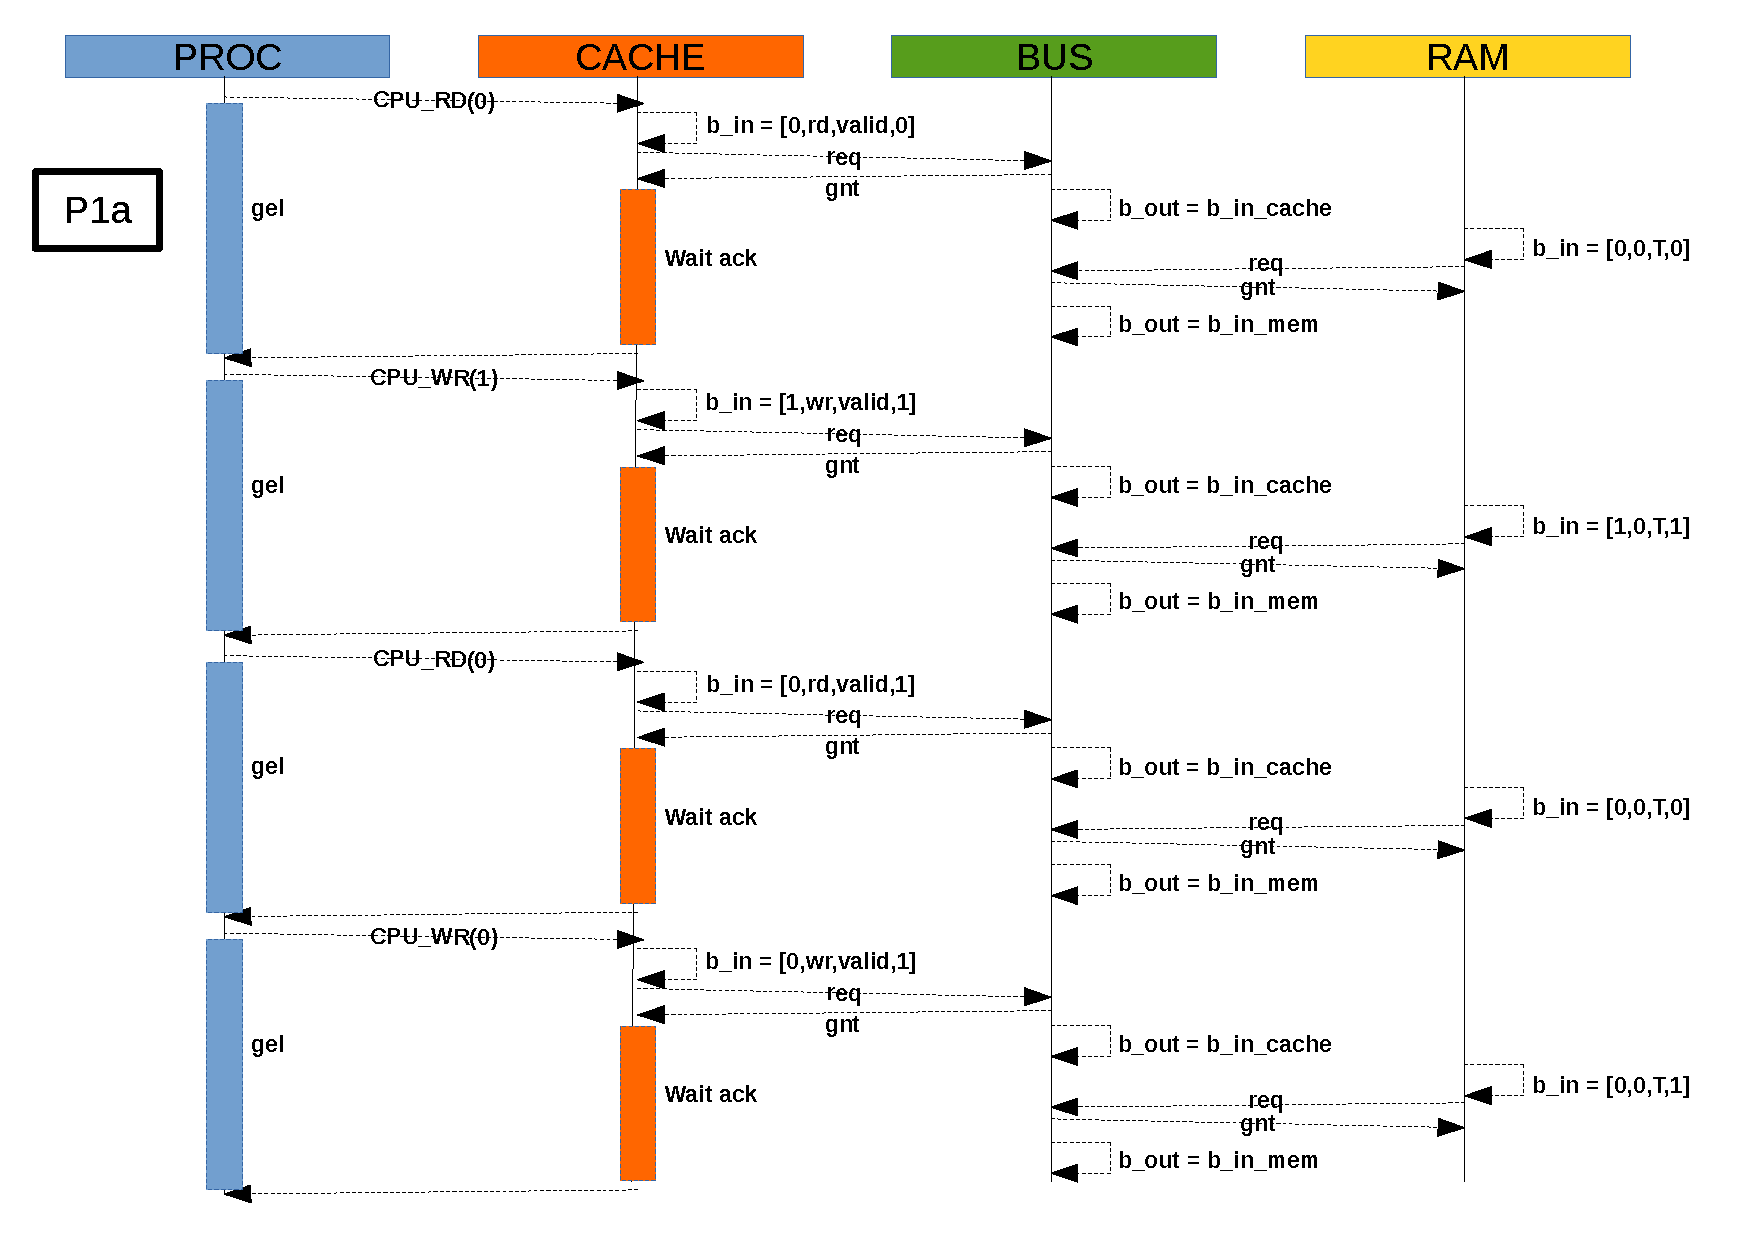
\includegraphics[scale=0.5]{images/seq1.pdf}}
\end{center}

\subsection{Architecture multi-processeur}
On présente ici les échages lors des exécutions de P1a et P2a. Pour alléger le
diagramme, chaque CPU est fusionné avec son cache, et les mises à jour internes
de chaque composant sont ommises.
\begin{center}
\centerline{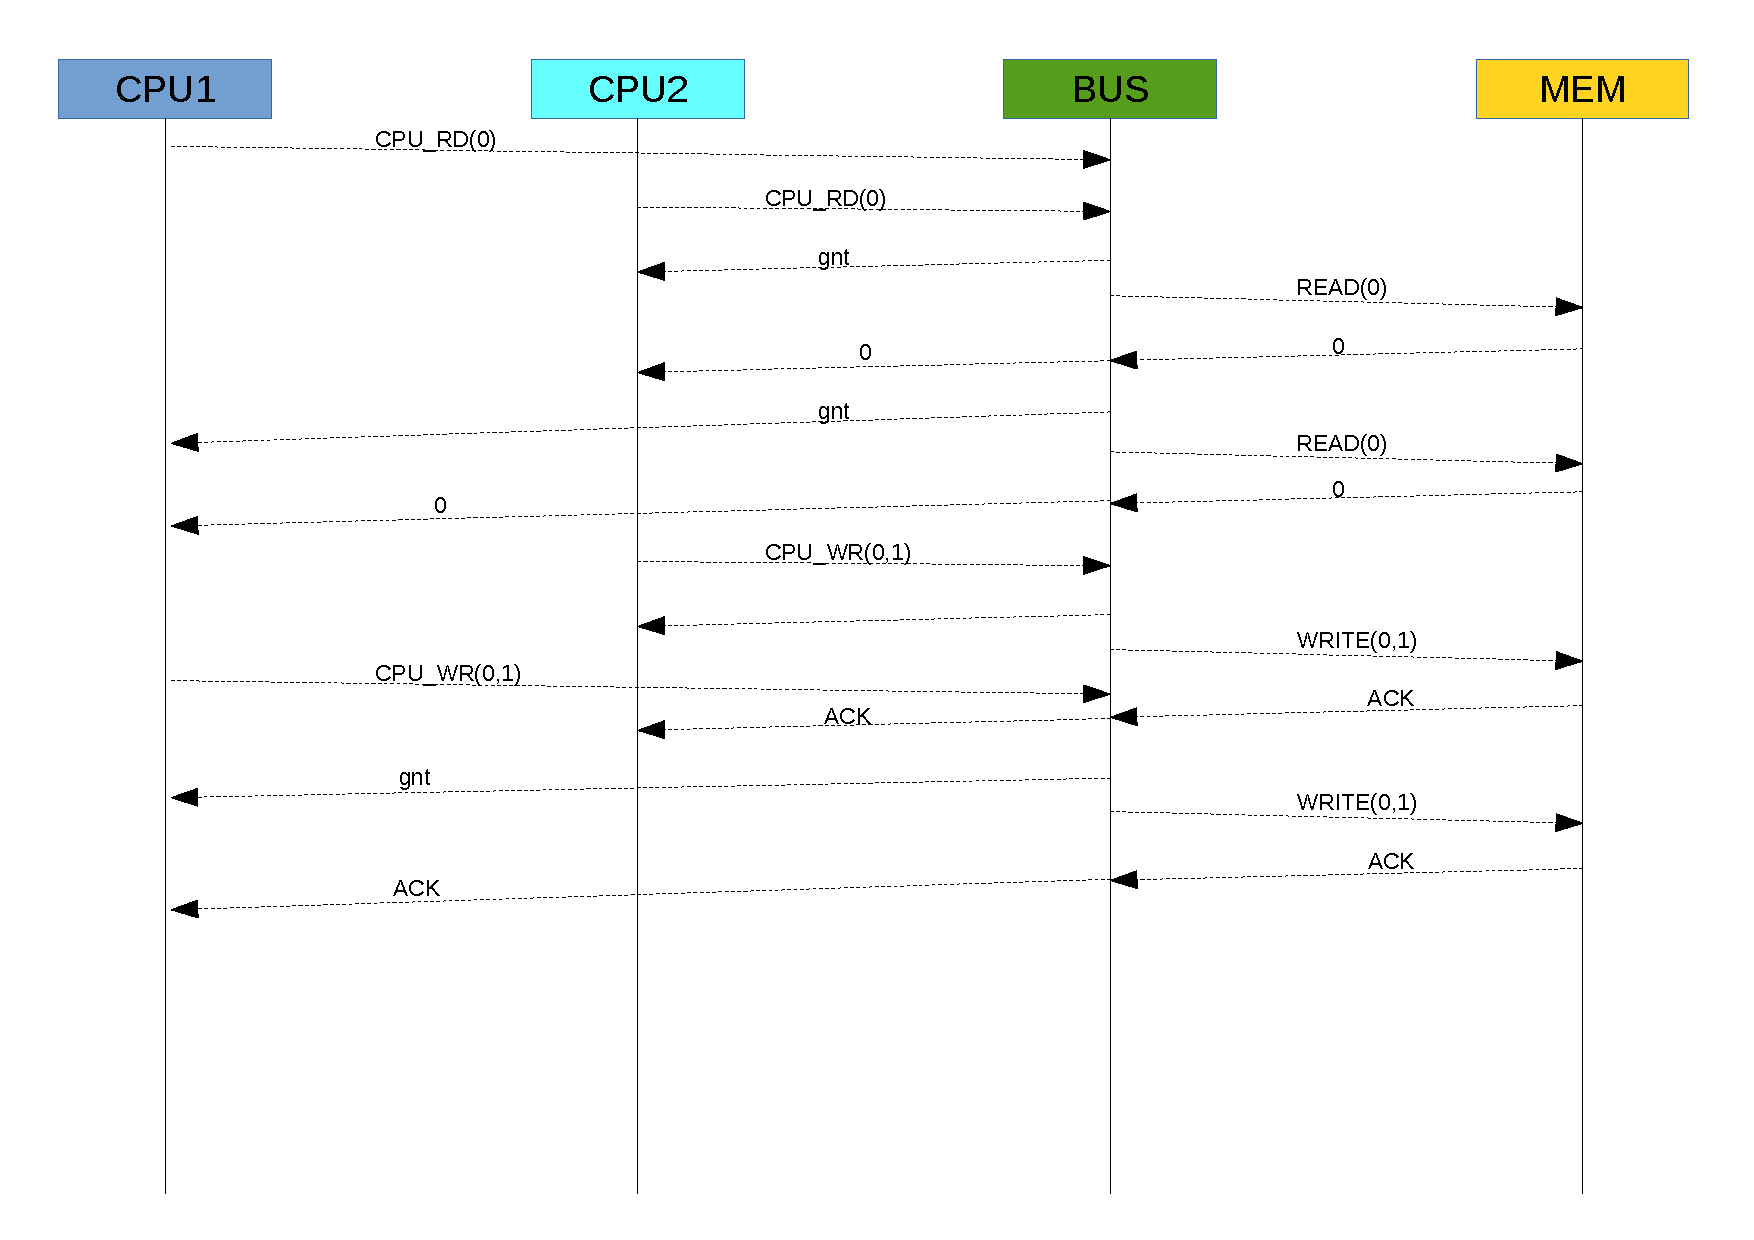
\includegraphics[scale=0.5]{images/seq2.pdf}}
\end{center}
Le mécanisme de SNOOP permet de conserver la cohérence des caches. En effet,
si un processeur A possède dans son cache la variable stockée à l'adresse X,
et que le processeur B écrit à l'adresse X, la valeur contenue dans le cache
de A ne sera plus à jour. Le SNOOP permet au cache de A de détecter une telle
écriture et se mettre à jour (ou invalider la ligne concernée). Ajouter à
cela un mécanisme d'écriture atomique (LL/SC par exemple) permet de garantir
des accès exclusifs à des données partagées.

\section{Interfaces entre composants}
Afin de modéliser cette architecture, il a tout d'abord fallu identifier le 
protocole de communication utilisé. Les composants communiqueront via les
signaux suivants (les canaux nommés \textit{b\_in} et \textit{b\_out} sont
des nappes de 4 fils [AD, CTRL, VALID, DT], \textit{arb\_gnt} un entier,
les autres sont booléens):
\begin{center}
\centerline{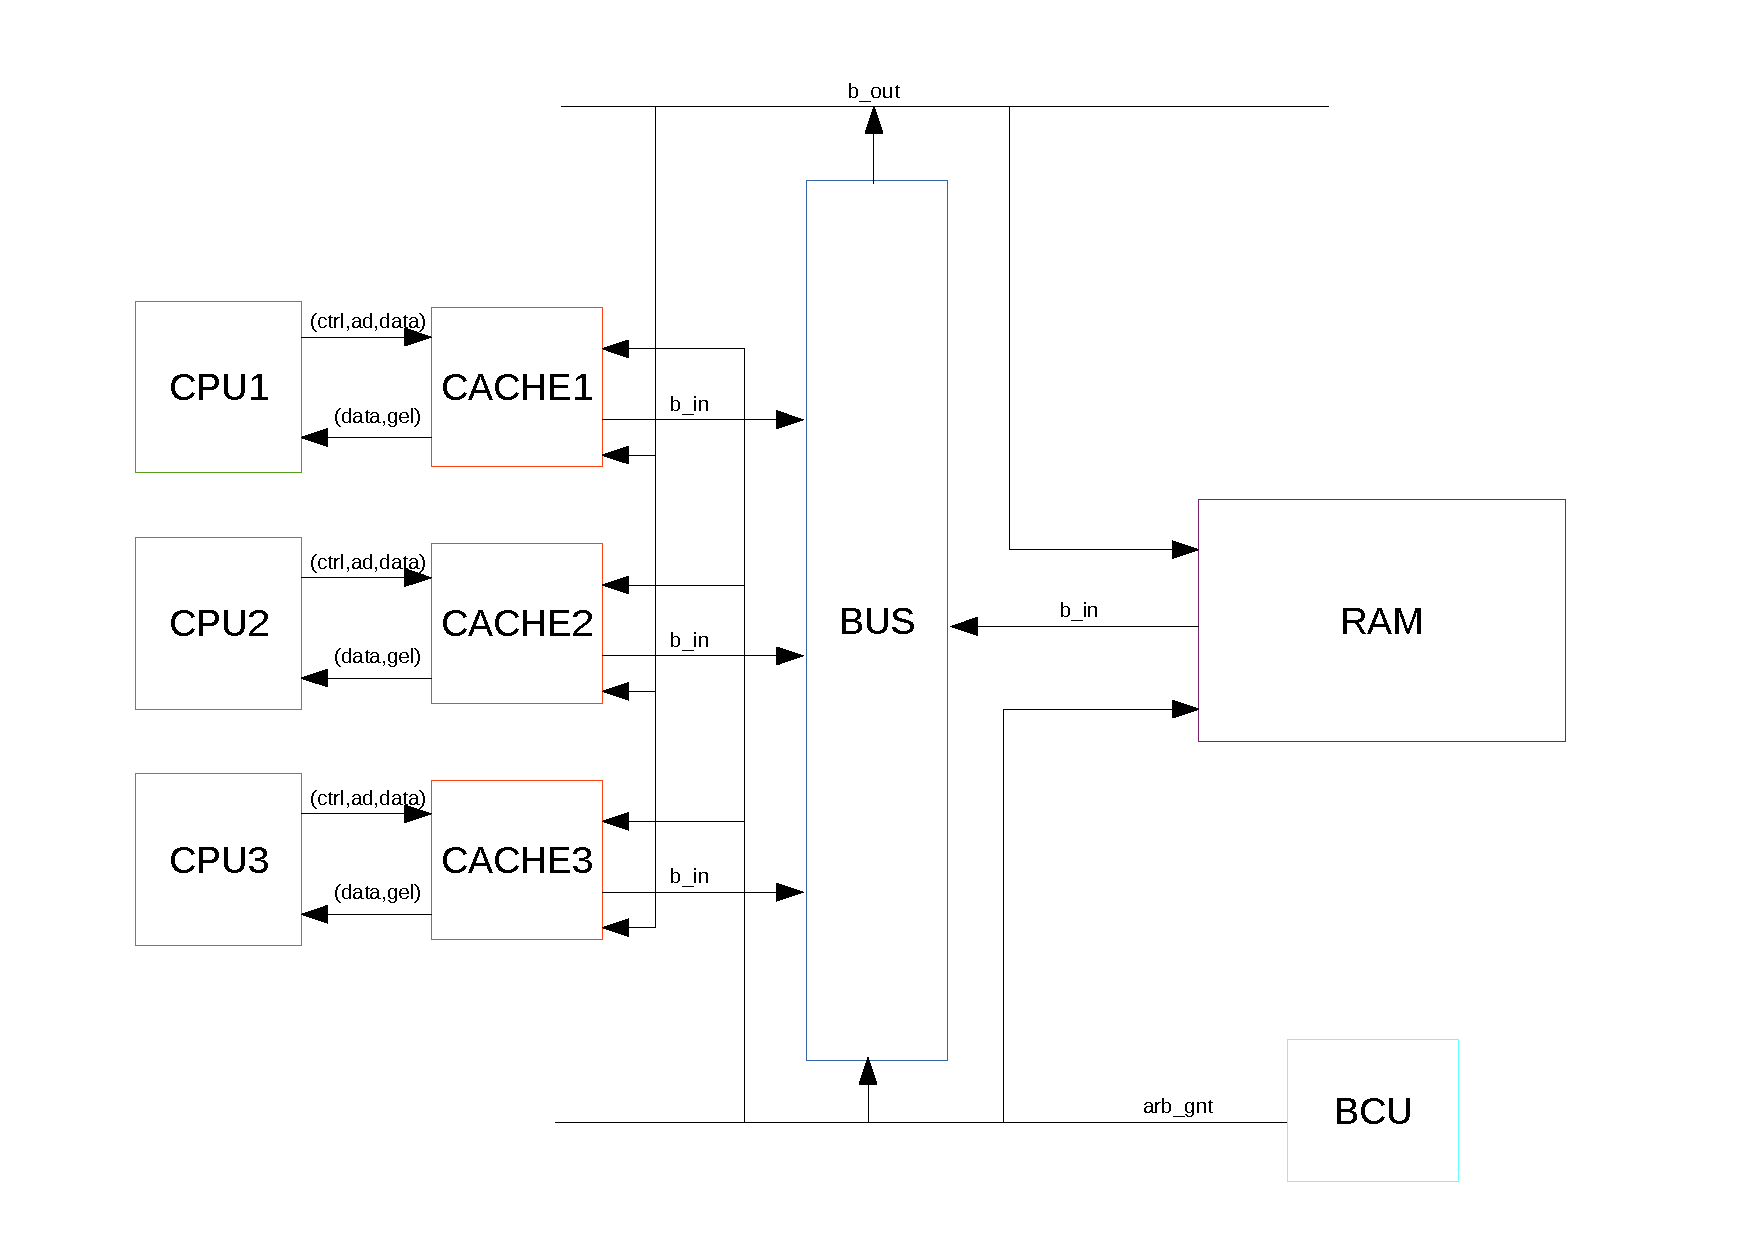
\includegraphics[scale=0.5]{images/archi.pdf}}
\end{center}

\section{Bus}
Le bus a pour rôle de copier la nappe issue d'un processeur ou de la mémoire
vers la nappe de sortie du bus, selon le maître déterminé par le BCU (signal
\texttt{arb\_gnt}). Il doit validé la propriété suivante :
\begin{itemize}
  \item si une requête d'un processeur passe sur le bus, elle sera immédiatement
    suivie d'une réponse de la mémoire
\end{itemize}

\section{Arbitre du bus (BCU)}
L'arbitre du bus (ou BCU) doit, à chaque cycle, déterminer si un maître souhaite
envoyer une requête sur le bus. S'il n'y a qu'une seule demande et que le bus est
libre, on donne le bus au maître faisant la demande. S'ils sont plusieurs, on
applique une stratégie pour élire le prochain utilisateur. Une stratégie de type
round-robin permet d'éviter les famines. Cependant, notre implantation n'utilise
pour le moment pas cette stratégie, mais donne l'accès au bus dans l'ordre de 
priorité suivant :
\[
MEM > CPU1 > CPU2 > CPU3 > NONE
\]
On obtient donc un chronogramme de ce type :
\begin{center}
\centerline{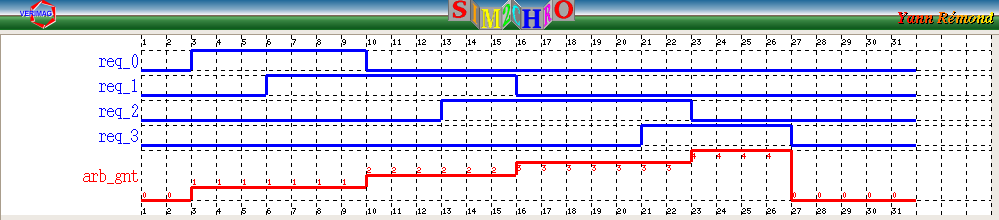
\includegraphics[scale=0.6]{images/bcu.png}}
\end{center}

\section{Processeur}
Le processeur prend en entrée un programme, ici simulé par les signaux suivants:
\begin{itemize}
  \item \texttt{op}: \textit{true} si écriture, lecture sinon;
  \item \texttt{valid}: \textit{true} si une instrution de type load ou store 
    est lue;
  \item \texttt{data\_in}: donnée à écrire si écriture;
  \item \texttt{ad}: adresse où lire/écrire en mémoire.
\end{itemize}
Il doit validé la propriété de vivacité suivante :
\begin{itemize}
  \item le processeur reviendra toujours à l'état non gelé
\end{itemize}
Dans l'implantation actuelle, cette propriété n'est pas vérifiée car le BCU
donne l'accès au bus toujours dans le même ordre. Une attribution par 
round-robin règlerait ce problème en supprimant les famines (voir code 
commenté du noeud bcu).
\begin{center}
\centerline{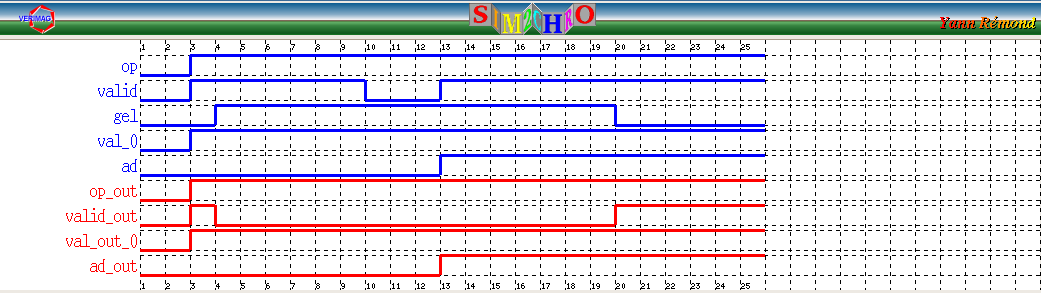
\includegraphics[scale=0.6]{images/proc.png}}
\end{center}


\section{Cache}
Le cache du processeur est modélisé sous la forme de l'automate suivant :
\begin{center}
\begin{tikzpicture}[->,>=stealth',shorten >=1pt,auto,node distance=4cm,
                    semithick]
  \tikzstyle{every state}=[fill=white,text=black]

  \node[state] (idle)                     {idle};
  \node[state] (rdmiss) [left of=idle]    {read\_miss};
  \node[state] (rdwait) [below of=rdmiss] {read\_wait};
  \node[state] (rdupd)  [below of=rdwait] {read\_update};
  \node[state] (wr)     [right of=idle]   {write};
  \node[state] (wrwait) [below of=wr]     {write\_wait};
  \path (idle)   edge [loop above] node {$(hit \bullet read)$}          (idle)
                 edge              node {$\overline{hit} \bullet read$} (rdmiss)
                 edge              node {$\overline{read}$}             (wr)
        (rdmiss) edge              node {$1$}                           (rdwait)
        (rdwait) edge [loop left]  node {$\overline{bus_{valid}}$}        (rdwait)
                 edge              node {$bus_{valid}$}                   (rdupd)
        (rdupd)  edge              node {$1$}                           (idle)
        (wr)     edge              node {$1$}                           (wrwait)
        (wrwait) edge              node {$bus_{valid}$}                   (idle)
                 edge [loop right] node {$\overline{bus_{valid}}$}        (wrwait);
        
\end{tikzpicture}
\end{center}
\paragraph{}On suppose que si aucune requête n'est reçue, on reste dans l'état
\texttt{idle}. De plus, l'état \texttt{write} fait la mise à jour du cache en
cas de \textit{hit} et envoie la requête sur le bus dans tous les cas. L'état 
\texttt{idle} renvoie la valeur en cache en cas de \textit{hit} sur une lecture
en un cycle.
\paragraph{}Le mécanisme de SNOOP a également été implanté. Le cache, lorsqu'il
n'utilise pas lui-même le bus, surveille les requêtes y passant. Si une requête
d'écriture sur une adresse faisant un \textit{hit} passe, il se met à jour avec
cette nouvelle valeur, afin de rester cohérent avec la mémoire.

\section{Mémoire}
La mémoire stocke l'état de variables à des adresses données. Pour simplifier
l'implantation et la vérification, on choisit une mémoire à 2 cases (adresse 
booléenne) pouvant prendre des mots de taille 1 bit (booléens). Cette mémoire
utilise le SNOOP pour détecter des requêtes la concernant sur le bus. Si elle
en détecte une, elle demande l'accès au bus à l'arbitre afin de répondre à
cette requête. \'Etant le maître le plus prioritaire, elle aura toujours
immédiatement accès au bus si elle le demande et qu'il est libre. On 
suppose également que la mémoire est extrêmement réactive et répond en un
cycle.
\begin{center}
\centerline{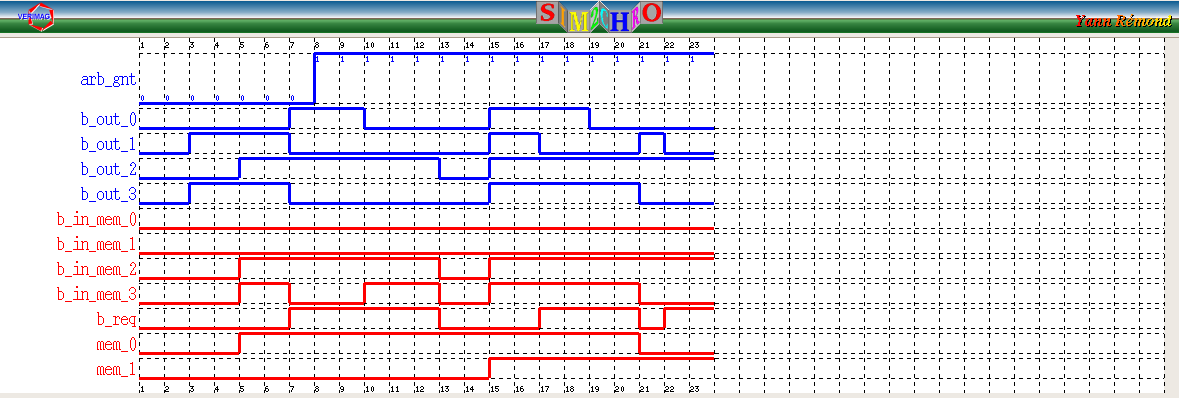
\includegraphics[scale=0.5]{images/mem.png}}
\end{center}

\section{Gestion de verrous}
L'ajout de la gestion des verrous afin de protéger des sections critiques
pose le problème des écritures atomiques. En effet, la prise d'un verrou se fait
en 2 étapes:
\begin{itemize}
  \item[1)] lecture du verrou en mémoire,
  \item[2)] si le verrou est libre, écrire en mémoire pour le prendre, sinon 
    recommencer
\end{itemize}
Cela pose cependant un problème : si deux processeurs A et B tentent de prendre
le verrou, l'enchainement suivant les fait tous deux entrer en section 
critique :
\[
A1 \rightarrow B1 \rightarrow A2 \rightarrow B2
\] 
En effet, ils vont tous deux lire la même valeur (verrou libre) et donc lancer
une écriture pour le prendre, chacun pensant être le seul à l'avoir. Il est
donc nécessaire d'avoir un mécanisme permettant de faire ces deux étapes de
manière atomique. On ajoute donc un nouveau type d'écriture permettant cela,
avec la stratégie LL/SC par exemple. Lors de la lecture (étape 1), le cache
va ``s'enregistrer'' localement, puis surveiller grâce au SNOOP les écritures
sur le verrou. Si lorsqu'il va exécuter l'étape 2, aucune écriture n'est passée,
il écrit et prend donc le verrou. S'il voit une écriture sur cette adresse avant
d'avoir pu le prendre, il se ``désenregistre'' et recommence à l'étape 1.
\end{document}
